\section{Negotiation Engineering}

\subsection{Concept}

\paragraph{Definitions}

\begin{itemize}
    \item \underline{Negotiation}: "A formal discussion with someone in order
        to reach an agreement"
    \item \underline{Engineering}: "The study of using scientific principles to design and build
        machines, structures, and other things"
    \item \underline{Engineering method}: "The strategy for causing the best
        change in a poorly understood or uncertain situation within the
        available resources." Characteristics:
        \begin{itemize}
            \item Solution oriented
            \item Looking for an answer (not the answer)
            \item In relation to existing constraints
            \item Valuating different options
            \item Mathematical language
            \item Heuristic techniques
                \begin{itemize}
                    \item Rule of thumb
                    \item Strategy
                    \item Trick
                    \item Simplification
                    \item Or any other mean reducing time needed to solve
                        a problem
                \end{itemize}
        \end{itemize}
    \item \underline{Negotiation Engineering}: "We define Negotiation Engineering
        as a solution-oriented approach to negotiation problems that uses
        quantitative methods in a heuristic way to find an adequate solution."
        It is an approach to bring scientific methods into practice and a sort
        of convex combination between "Game theory" and "Harward method".
\end{itemize}

\paragraph{The Method}

Application of engineering method/reasoning to negotiation. It is based
on four principles:
\begin{enumerate}[a.]
    \item Decomposition
        \begin{itemize}
            \item Division in sub and sub-sub problems
            \item Reduction of complexity
            \item Allow identification of underlying key problems
        \end{itemize}
    \item Formalization
        \begin{itemize}
            \item Translation of critical sub-problem into mathematical language
            \item Thereby: reduction of problem to its most formal structure
        \end{itemize}
    \item Mathematical Method
        \begin{itemize}
            \item If the problem is stated in mathematical language one can
                access a variety of existing mathematical tools:
                \begin{itemize}
                    \item game theory
                    \item mathematical optimalization
                    \item statistics
                    \item etc.
                \end{itemize}
        \end{itemize}
    \item Heuristics
        \begin{itemize}
            \item Experience-based techniques
            \item Not guaranteed to be obtimal
            \item But good enough for the given situation
        \end{itemize}
\end{enumerate}

\paragraph{Illustration}
Brexit negotiation with negotiation engineering

\begin{figure}[h]
    \centering
    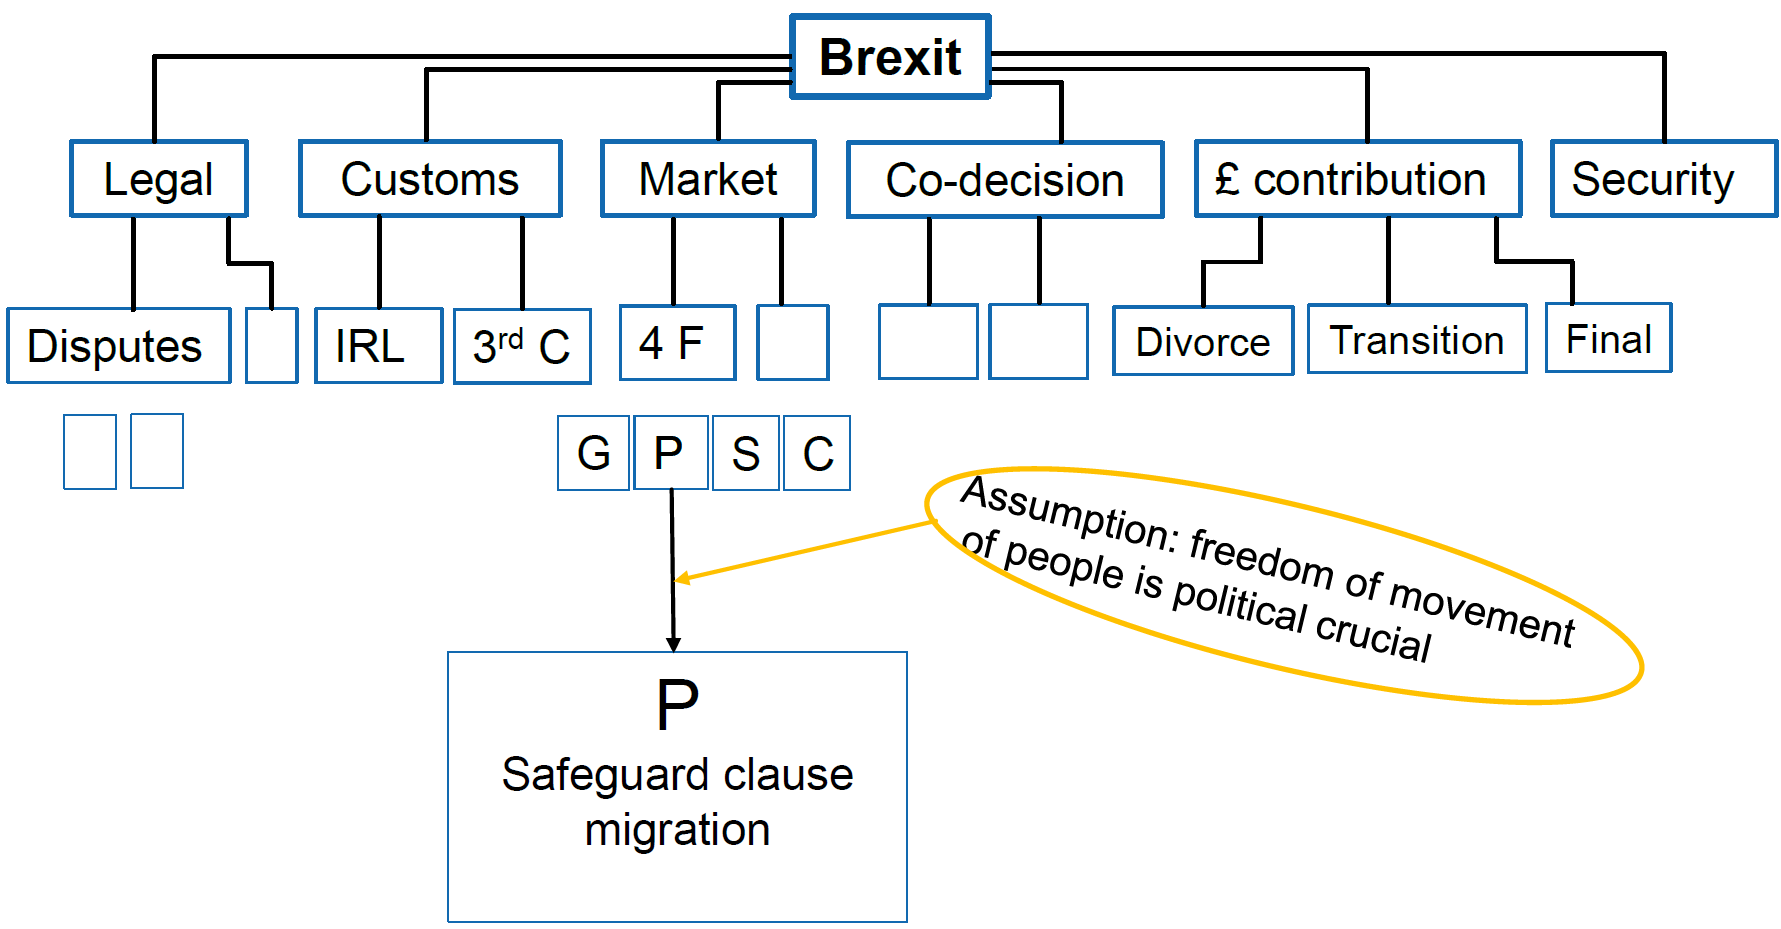
\includegraphics[width=0.6\textwidth]{Pictures/Brexit.png}
\end{figure}

\subparagraph{Safeguard Clause Migration}

\begin{itemize}
    \item Possible model that combines the EU free movement of persons
        principle with the ability to regulate the flow of migration
        in specific cases.
    \item Inspired by the abstract existing safeguard clause [Art. 14(2)] in
        the bilateral agreement Switzerland-EU.

        \vspace{1\baselineskip}

        Article 14 - Joint Committe

        In the event of serious economic or social difficulties, the
        Joint Committee shall meet, at the request of either Contracting
        Party, to examine appropriate measures to remedy the situation.
        The Joint Committee may decide what measures to take within
        $60$ days of the date of the request. This period may be extended by
        the Joint Committee. The scope and duration of such measures shall
        not exceed that which is strictly necessary to remedy the situation.
        Preferences shall be given to measures that least disrupt the
        working of this Agreement.

    \item A more concrete safeguard clause could be formulated.
    \item In the form of a clear trigger and well described measures.
\end{itemize}

\subparagraph{On the Trigger}

\begin{itemize}
    \item If the net migration is significantly higher than the average, the
        safeguard clause will be triggered.
    \item This trigger point could be defined by the following formula:
        \begin{align*}
            d_i = m + \alpha_i \beta_i \gamma_i 2 \sigma
        \end{align*}
        with $m=$ average migration, $\alpha_i =$ current relative number
        of EU citizens in state $i$, $\beta_i =$ current relative number
        of third country citizens, $\gamma_i =$ unemployment factor and
        $2 \sigma = 2 \cdot$ standard deviation
    \item If the net migration of the country is larger than $d_i$, the
        safeguard clause is triggered.
\end{itemize}

\subparagraph{As an Example}

Net migration "EU-25" per 1000 inhabitants:
\begin{itemize}
    \item Threshold UK: $148'824$
    \item Actual UK: $160'421$
    \item UK would have been allowed to activate safeguard clause because
        actual migration is larger than threshold.
\end{itemize}


\paragraph{Generalizability of Negotiation Models}

\begin{itemize}
    \item A key issue in the study of negotiations is the analysis of
        commonalities across different negotiation contexts and the
        question to what extend an approach can be generalized and
        applied to different negotiation cases.
    \item To contribute to this objective, abstract models are used to
        draw general conclusions about generic negotiation situations.
    \item Mathematics provides a powerful instrument for modeling complex
        problems. However, if such models remain on a high level of abstractness,
        their usefulness in complicated real-world negotiations is often reduced.
    \item Illustration with a generalized formulation of a "give-and-take"
        negotiation in the form of a mathematical program.
    \item In the negotiation, the actors want to find a common solution
        that ideally maximizes a combination of the utility function, a sort of
        joint welfare function.
    \item Nash proposed a convincing concept in the form of a mathematical
        program: maximize the product of the utilities, which are subject to
        the negotiation set (Pareto optimal and above levels).
    \item Maximize a function, subject to a set of constraints. Nash proved:
        this solution satisfies four axioms that define a reasonable
        negotiation solution.
    \item We generalize Nash's Bargaining solution with his concept of a
        combined utility function $F_p$, and model the negotiation as
        follows:
        \begin{itemize}
            \item A number of $\overline{a}$ actors ($\overline{a} \geq 2$)
                negotiate over a set of issues $I=\geschwungeneklammer{i \ | \ i=1,\dots,\overline{i}}$
            \item We assume that the actors agree to split the complex negotiation
                into $\overline{p}$ phases ($p = 1,\dots,\overline{p}$), in each of
                which a part of the issue $I_p \subseteq I$ is negotiated and brought
                to a conclusion.
            \item For all the different issues $i$, each actor has a utility
                function $u_{a,i}$
            \item Each actor has a set of constraints $C_a$ limiting his scope
                of actions and defining the area of a possible solution for
                actor $a$.
            \item The intersection of all constraints $C_a$ forms a zone of
                possible agreement (ZOPA), where the solution of the
                negotiation problem must be an element of the feasible region
                $C_1 \cap \dots \cap C_a$
            \item In a world or rational, far-sighted actors, each actor $a$ tries
                to maximize his or her utility $u_{p a}$ in every phase $p$.
                The utility of actor $a$ in phase $p$ is $u_{p a} =
                \sum_{i=1}^{\overline{i}} \beta_{a,i} u_{a,i} \ , \ i \in I_p$,
                where $\beta_{a,i}$ is a weighting factor, weighting the
                importance of issue $i$ for actor $a$.
            \item Model of Nash's concept of combined utility function $F_p$
                \begin{align*}
                    \max &F_p (u_{p1},\dots,u_{pa},\dots,u_{p \overline{a}})
                    \\
                    \text{s.t. } &u_{pa} \geq u_{pa}^{sec} \ \forall a
                    \\
                    &u_{p1},\dots,u_{pa},\dots,u_{p \overline{a}} : \text{Pareto}
                \end{align*}
                where
                \begin{align*}
                    &F_p (u_{p1},\dots,u_{pa},\dots,u_{p \overline{a}}) = \prod_{a=1}^{\overline{a}} (u_{pa} - \alpha_a u_{pa}^{sec})
                    \\
                    &\alpha_a \text{ is a weighting factor, weighting the importance of actor } a
                    \\
                    &u_{pa}^{sec} \text{ is security level of actor $a$ in phase } p
                \end{align*}
            \item As soon as all phases are completed, each actor checks the overall
                result and, if not satisfied, asks to re-negotiate the crucial phase
                until eventually everything is agreeable $\rightarrow$ iterative
                process
        \end{itemize}
    \item Even though this process could go through many iterations in
        theory, in practice, the time consuming and burdensome re-opening of
        a closed phase does not often happen (e.g., in EU membership negotiations,
        where closed chapters [phases] are rarely re-opened).
    \item This is a processing combining advantages of a sequential and simultaneous
        resolution of issues when (i) the number of issues is too large to be
        negotiated at once, but (ii) the combination of different issues (which
        are different valuated by the actors) allows to trade them off against
        each other $\rightarrow$ logrolling/cross-concessions.
    \item This principle 'nothing is agreed until everything is agreed' allows
        a re-negotiation of already-concluded phases if the overall result
        should not satisfy one of the actors. In practice, the acceptance of a
        'not so perfect' result in a previous phase can act as a bargaining
        chip in later phases.
\end{itemize}

\subparagraph{Difficulties in complex negotiations}

\begin{itemize}
    \item Difficult to precisely define the different utility functions
    \item The mathematical programming problem remains almost unsolvable
        (the feasible regions are not necessarily convex, and the utility
        functions are often not even continuous).
    \item $\Rightarrow$ Negotiation Engineering tries to overcome these
        difficulties in real-world application
\end{itemize}

\subsection{Strenghts and weaknesses of Negotiation Engineering}

\paragraph{Strenghts}

\begin{itemize}
    \item Revealing the underlying mechanism with mathematical tools.
    \item Define abstract mechanism without pre-imposing the outcome
    \item De-emotialization of the problem
\end{itemize}

\paragraph{Weaknesses}

\begin{itemize}
    \item It does not concentrate on higher-level factors: it is not strategic,
        but ("only") technical; no higher-level discussions
    \item It is not about the search of the answer to a general question
    \item Formalization is a reduction (leaving out some aspects)
    \item Not all problems can be quantified
\end{itemize}


